\chapter{Simulations}
\minitoc
\thispagestyle{plain}
\def\saltino{\vspace{0.5cm}}

In this chapter we will see the implementation of part of the system using Matlab/Simulink platform. Some results are shown. Implementation takes into account the presence of noise in ARTVA receiver and consider a good estimation for the position and attitude of the system. To make simulation faster, we used \texttt{C--compiled} functions to perform heavier computational tasks\marginnote{The complete project is available on--line as a public Github repository. Please refer to the project for the actual source code of the single blocks.}. 

\section{Implementations}

\subsection{Dynamic model}

The dynamic of the model is implemented with an \texttt{S-Function}, while the control is derived from the linearization of the model and thus inserted as gain in the model loop. The system has a free $\vrz$ attitude, while position is controlled through the use of an integrated velocity vector.
\begin{figure*}[h] \centering
\begin{tikzpicture}[auto,node distance=10mm and 7mm, >=latex']

	\node [block, fill=gray!40] (hexamodel) {Hexacopter Model};
	\fromworkspace{parameter}{\scriptsize{Parameters}}{at=(hexamodel),xshift=-50,yshift=30}
	\node [sum, left=of hexamodel] (sumA) {$+$};
	\node [block, left=of sumA] (force) {$F_i = \dfrac{mg}{6}$};
	
	\node [ellipse, draw, minimum width=1.3cm, above=of force] {\scriptsize{Time}};
	\node [block,below=of hexamodel] (controller) {LQR Controller};
	\node [block, right=of controller] (integrator) {$\dfrac{1}{s}$};
	\fromworkspace{zattitude}{\scriptsize{$\hat{\mathbf{z}}$ attitude}}{at=(controller),yshift=-30,xshift=-50}
	\node [sum, right=of integrator] (sumB) {$+$};
	\node [block, right=of sumB, text width=2cm,align=center] (searching) {Searching Algorithm};
	\node [block, below=of searching, text width=2cm,align=center] (obstacle) {Obstacle Avoiding};
	\coordinate[at=(hexamodel),xshift=220] (intersection);
	\toworkspace{results}{$\mathbf{x}$}{right=of intersection};

	\draw [->] (force) -- (sumA);
	\draw [->] (sumA) -- (hexamodel);
	\draw [->] (hexamodel) -- (results_in);
	\draw [->] (searching) -- (sumB);
	\draw [->] (sumB) -- (integrator);
	\draw [->] (integrator) -- (controller);

	\draw [->] (controller) -| (sumA);
	\draw [->] (zattitude_out) -| (controller);
	\draw [->] (parameter_out) -| (hexamodel);
	\draw [->] (obstacle) -| (sumB);
	\draw [->] (intersection) |- (searching);
	\draw [->] (intersection) |- (obstacle);

\end{tikzpicture}
\caption{System complete model}
\end{figure*}
\saltino

\begin{figure*}[h] \centering
\begin{tikzpicture}[auto,node distance=10mm and 7mm, >=latex]
	\inputpin{stato}{$\mathbf{x}$}{}
	\draw [at=(stato), xshift=50, fill=black] ++(0,0) node(muxin){} -- ++(0,2cm) -- ++(1mm,0) -- node[pos=0.2](posizione){} node[pos=0.4](velocita){} node[pos=0.6](angolo){} node[pos=0.8](velrotazione){} ++(0,-4cm) -- ++(-1mm,0) -- cycle;
	\node [sum, at=(posizione), xshift=50] (sumA) {$+$};
	\node [sum, at=(angolo), xshift=100] (sumB) {$+$};
	\draw [at=(stato), xshift=200+1mm, fill=black] ++(0,0) node(muxout){} -- ++(0,2cm) -- ++(-1mm,0) -- node[pos=0.2](posizioneB){} node[pos=0.4](velocitaB){} node[pos=0.6](angoloB){} node[pos=0.8](velrotazioneB){} ++(0,-4cm) -- ++(1mm,0) -- cycle;
	\node [gain,at=(stato.west), xshift=255, regular polygon rotate=-90] (gain) {$K$};
	\outputpin{controllo}{$\mathbf{u}$}{at=(stato.west), xshift=315};

	\inputpin{refer}{$\mathbf{x}_f$}{at=(stato.center), yshift=-80}
	\inputpin{attitz}{$\psi_f$}{at=(stato.center), yshift=-110}

	\draw [->] (stato_out) -- (muxin.center);
	\draw [->] (posizione.west) -- node[text width=1.5cm,align=left,pos=0.60]{\scriptsize{Position}} (sumA.west);
	\draw [->] (sumA.east) -- (posizioneB.west);
	\draw [->] (velocita.west) -- node[text width=1.5cm,align=left,pos=0.175]{\scriptsize{Velocity}} (velocitaB.west);
	\draw [->] (angolo.west) -- node[text width=1.5cm,align=left,pos=0.275]{\scriptsize{Attitude}} (sumB.west);
	\draw [->] (sumB.east) -- (angoloB.west);
	\draw [->] (velrotazione.west) -- node[text width=1.5cm,align=left,pos=0.175]{\scriptsize{Ang.ratio}} (velrotazioneB.west);
	\draw [->] (muxout.center) -- (gain);
	\draw [->] (gain) -- (controllo_in);

	\draw [->,draw=white,line width=2] (refer_out) -| (sumA.south);
	\draw [->,draw=white,line width=2] (attitz_out) -| (sumB.south);
	\draw [->] (refer_out) -| node[right,at end]{$-$} (sumA.south);
	\draw [->] (attitz_out) -| node[right,at end]{$-$} (sumB.south);

\end{tikzpicture}
\caption{Tracking problem}
\end{figure*}
\saltino
\FloatBarrier

\subsection{Receiver Model}

The receiver implements a mean sampler to reduce white Gaussian noise. The model of the receiver contains the equations of the H--field at which noise proportional to signal intensity on each antenna. The idea is to get \num{40}\si{\decibel} of signal to noise ratio, that is quite optimistic, but it is also the value declared from some manufacturer. Also algorithm may work with lower receiver SNR.
\begin{figure*}[h] \centering
\begin{tikzpicture}[auto,node distance=10mm and 10mm, >=latex]
	
	\inputpin{stato}{$\mathbf{x}$}{}
	\node [block, right=of stato_out,fill=gray!40] (Hfield) {$\mathbf{H}\left( \mathbf{x}, \mathbf{p}_T, \hat{\mathbf{m}} \right)$};
	\fromworkspace{mvector}{\scriptsize{Magnetic Dipole $\hat{\mathbf{m}}$}}{at=(Hfield),xshift=-60,yshift=30,text width=2.7cm}
	\fromworkspace{tpos}{\scriptsize{Transmitter position $\mathbf{p}_T$}}{at=(Hfield),xshift=-60,yshift=50,text width=2.7cm}

	\coordinate [right=of Hfield] (intersection);
	\node [block, below=of intersection,text width=1cm, align=center] (absolute) {$|\mathbf{H}|$};
	\node [sum, below=of absolute] (prod) {$\times$};
	\node [block, left=of prod] (noise) {$\mathcal{N}(\mathbf{0},\Sigma)$};
	\node [gain, right=of prod, regular polygon rotate=-90, text width=0.3cm] (gain) {\scriptsize{SNR}};
	\node [sum, at=(intersection), xshift=100] (somma) {$+$};
	\outputpin{hvalue}{$\mathbf{H}$}{right=of somma}

	\draw[->] (stato_out) -- (Hfield);
	\draw[->] (Hfield) -- (somma);
	\draw[->] (somma) -- (hvalue_in);
	\draw[->] (intersection) -- (absolute);
	\draw[->] (absolute) -- (prod);
	\draw[->] (noise) -- (prod);
	\draw[->] (prod) -- (gain);
	\draw[->] (gain) -| (somma);
	\draw[->] (mvector_out) -| (Hfield);
	\draw[->] (tpos_out) -| (Hfield);

\end{tikzpicture}
\caption{Receiver implementation}
\end{figure*}
\saltino
\FloatBarrier

\subsection{Obstacle avoidance}

In the obstacle avoidance block we find a model of the receivers, written as a \texttt{mex--function}, and than the quite simple algorithm that allow us to avoid the obstacle generating a velocity vector orthogonal to the obstacle plane. This velocity vector is added to the searching input. This behavior is typical of the grounded paradigm.
\begin{figure*}[h] \centering
\begin{tikzpicture}[auto,node distance=10mm and 7mm, >=latex]
	\inputpin{stato}{$\mathbf{x}$}{}
	\coordinate [right=of stato_out] (intersectionA);
	\node [block, right=of intersectionA,fill=gray!40] (range_finder) {Range Finder Model ${d_i}$};
	\fromworkspace{punti}{\scriptsize{${\Psi = [\mathbf{x}_i:i=1..M]}$}}{at=(range_finder),xshift=-60,yshift=30,text width=2cm}
	\fromworkspace{parametri}{\scriptsize{$[h,\,\rho]$}}{at=(range_finder),xshift=-60,yshift=50,text width=2cm}
	\node [block, below=of range_finder] (rotmat) {${\mathcal{R}^T(\phi,\theta,\psi)}$};
	\node [block, right=of range_finder] (velocita) {${\mathbf{v}_b = \sum\limits_{i=1}^{6} v(d_i) \hat{\mathbf{u}}_i}$};
	\node [sum, right=of velocita] (prod) {$\times$};
	\outputpin{velout}{$\mathbf{v}$}{right=of prod}
	\fromworkspace{paramV}{\scriptsize{$[p_1,\,p_2,\,p_3]$}}{at=(velocita),xshift=-45,yshift=30}

	\draw [->] (stato_out) -- (range_finder);
	\draw [->] (range_finder) -- (velocita);
	\draw [->] (velocita) -- (prod);
	\draw [->] (prod) -- (velout_in);
	\draw [->] (intersectionA) |- (rotmat);
	\draw [->] (rotmat) -| (prod);
	\draw [->] (punti_out) -| (range_finder);
	\draw [->] (parametri_out) -| (range_finder);
	\draw [->] (paramV_out) -| (velocita);

\end{tikzpicture}

\caption{Obstacle avoidance sub--block}
\end{figure*}
\saltino
\FloatBarrier

\subsection{Searching algorithm}

The receiver output feeds directly the two component of the source searching algorithm. The field information is transformed in an intensity and in a direction value to get an exploration direction. Measured field is used to perform the emulation, as an optimization problem. It was quite tricky to call the optimizer from Simulink, but possible using the \texttt{caller extrinsic} directive, alongside with an external evaluation from the Matlab engine, using \texttt{feval}. To speed up the process, residuals and barrier function results are evaluated using a \texttt{mex--function}. The parzen window estimation is performed offline, only as qualitative expression of the quality of the algorithm. The system shows some problem due to the symmetry of the transmitting field.
\begin{figure*}[h] \centering
\begin{tikzpicture}[auto,node distance=10mm and 7mm, >=latex]
	\inputpin{stato}{$\mathbf{x}$}{}
	\coordinate [right=of stato_out] (intersectionA);
	\node [block, right=of intersectionA] (Hfield) {$\mathbf{H}$ sensor};
	\fromworkspace{mvector}{\scriptsize{Magnetic Dipole $\hat{\mathbf{m}}$}}{at=(Hfield),xshift=-60,yshift=30,text width=2.7cm}
	\fromworkspace{tpos}{\scriptsize{Transmitter position $\mathbf{p}_T$}}{at=(Hfield),xshift=-60,yshift=50,text width=2.7cm}
	\coordinate [right=of Hfield] (intersectionB);
	\node [block, right=of intersectionB] (direction){$\begin{array}{l} |\mathbf{H}| \\ \cos(\theta) \\ \sin(\theta) \end{array}$};
	\node [block, right=of direction] (filtering) {$\dfrac{\alpha_1 s + 1}{\beta_1 s^2 + \beta_2 s +1}$};
	\node [block,right=of filtering,text width=2cm,align=center] (velocity) {Exploration direction};
	\outputpin{velout}{$\mathbf{v}$}{right=of velocity}
	\node [block,below=of filtering,fill=gray!40,text width=3cm,align=center, minimum height=2cm] (emulation) {Emulation ${(\mathbf{H} - \hat{\mathbf{H}})^2 = \mathbf{0}}$};
	\coordinate [at=(emulation.east), yshift=15] (emulation_out1);
	\coordinate [at=(emulation.east), yshift=-15] (emulation_out2);
	\coordinate [at=(emulation.west), yshift=15] (emulation_in1);
	\coordinate [at=(emulation.west), yshift=-15] (emulation_in2);

	\toworkspace{posopt}{Optimized $\mathbf{p}_T$}{right=of emulation_out1}
	\toworkspace{mopt}{Optimized $\hat{\mathbf{m}}$}{right=of emulation_out2}
	\fromworkspace{paramV}{\scriptsize{Parameters}}{at=(velocity),xshift=-45,yshift=30}

	\draw [->] (mvector_out) -| (Hfield);
	\draw [->] (tpos_out) -| (Hfield);
	\draw [->] (stato_out) -- (Hfield);
	\draw [->] (Hfield) -- (direction);
	\draw [->] (direction) -- (filtering);
	\draw [->] (filtering) -- (velocity);
	\draw [->] (velocity) -- (velout_in);
	\draw [->] (intersectionA) |- (emulation_in2);
	\draw [->] (intersectionB) |- (emulation_in1);
	\draw [->] (emulation_out1) -- (posopt_in);
	\draw [->] (emulation_out2) -- (mopt_in);
	\draw [->] (paramV_out) -| (velocity);
\end{tikzpicture}

\caption{Searching algorithm sub--block}
\end{figure*}
\saltino
\FloatBarrier

\section{Results}
In the next pages some results are reported, for a sample simulation.

\begin{figure*}[f]
	\centering
	\includegraphics[]{ch4/img/3Dplot.pdf}
\label{fig:3dplot}
\caption{Graphical representation of a searching mission. The blue part is an obstacle, while the red dot is the position of the transmitter.}
\end{figure*}

\begin{figure*}[f]
	\centering
	\includegraphics[]{ch4/img/State.pdf}
\label{fig:state}
\caption{State of the drone during the entire searching routine. The earlier seconds are used to stabilize the drone, while for the rest of the time tries to reach the source.}
\end{figure*}

\begin{figure*}[f]
	\centering
	\includegraphics[]{ch4/img/Searching.pdf}
\label{fig:searching}
\caption{The searching routine perceived value. It is important to notice the monotonic behavior of the H--field strength. The algorithm succeeds in finding the direction in which the field increases.}
\end{figure*}

\begin{figure*}[f]
	\centering
	\includegraphics[]{ch4/img/ParzenWindow.pdf}
\label{fig:parzwin}
\caption{The results for the emulation routine. We can see that this algorithm does not produce great result at this time. Wee need to infer some more knowledge to the emulation equations. This problem could be related to the intrinsic symmetry of the field.}
\end{figure*}

\begin{figure*}[f]
	\centering
	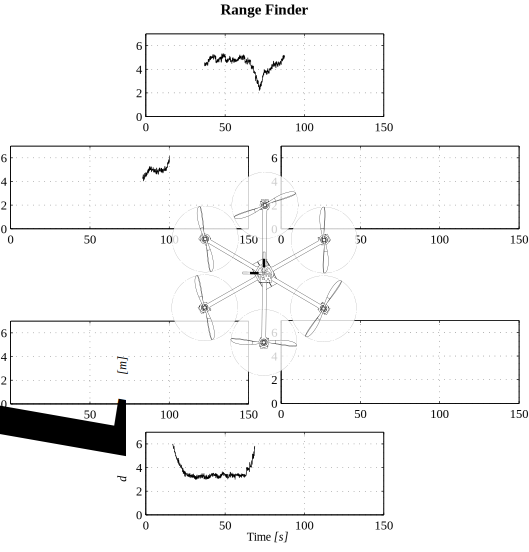
\includegraphics[]{ch4/img/RangeFinder.pdf}
\label{fig:rangefinder}
\caption{The range finder distance reading.}
\end{figure*}

